\documentclass[a4paper,10pt]{article}
\usepackage[utf8]{inputenc}
%\usepackage[francais]{babel}
\usepackage[T1]{fontenc}
\usepackage{graphicx}
\usepackage{eurosym}
\usepackage{verbatim}
\usepackage{amsmath, amsthm}
\usepackage{latexsym}
\usepackage{amssymb}
\usepackage{tabularx}
\usepackage{setspace}
\usepackage{listings}
\usepackage{geometry}
\usepackage{fancyhdr}
%\usepackage{enumitem}
\usepackage{colortbl}
%\usepackage[dvipsnames]{xcolor}
\usepackage{booktabs}
%\usepackage{moreverb}

%\usepackage{cite}
\DeclareMathAlphabet{\mathonebb}{U}{bbold}{m}{n}
\newcommand{\one}{\ensuremath{\mathonebb{1}}}

\usepackage{color}
%\usepackage{multirow}
%\usepackage{float}
\definecolor{gris25}{gray}{0.75}
\usepackage{colortbl}
\usepackage{fancyhdr}
\usepackage{amsmath,amsfonts,amssymb}
%\usepackage{titlesec}
%\usepackage{supertabular}
\usepackage{longtable}

\usepackage{caption}
\usepackage{subcaption}


\usepackage{listings}
\definecolor{dkgreen}{rgb}{0,0.4,0}
\definecolor{gray}{rgb}{0.5,0.5,0.5}
\definecolor{mauve}{rgb}{0.58,0,0.82}


\usepackage[numbers]{natbib}

\newcommand\Mycite[1]{%
  \citeauthor{#1}~(\citeyear{#1})~\cite{#1}}


\usepackage{multicol}
\usepackage{graphicx}

%\usepackage{algorithm2e}

% marges,etc.
%\usepackage{a4wide}
\hoffset -1cm
\voffset -2cm
\textheight 25cm
\headheight 1cm
\headsep 1cm
\topmargin 0cm
\textwidth 16cm

%to change temporaly a margin
\def\changemargin#1#2{\list{}{\rightmargin#2\leftmargin#1}\item[]}
\let\endchangemargin=\endlist 


%pour les couleurs
\usepackage{color}
\definecolor{mycolor}{rgb}{0.06,0.32,0.39}

%liens dans le corps du texte
\usepackage{hyperref}
\hypersetup{
    colorlinks=true,
    linkcolor=blue,
    citecolor=dkgreen,
    filecolor=blue,
    urlcolor=blue,
}

\urlstyle{same}

\definecolor{dkyellow}{cmyk}{0, 0, 0.2, 0}
\lstset{
  language=Python,                % the language of the code
  basicstyle= \footnotesize,      % the size of the fonts that are used for the code
  numbers=left,                   % where to put the line-numbers
  numberstyle=\tiny\color{gray},  % the style that is used for the line-numbers
  stepnumber=2,                   % the step between two line-numbers. If it's 1, each line
                                  % will be numbered
  showspaces=false,               % show spaces adding particular underscores
  showtabs=false,                 % show tabs within strings adding particular underscores
  frame=single,                   % adds a frame around the code
  rulecolor=\color{black},        % if not set, the frame-color may be changed on line-breaks within not-black text (e.g. commens (green here))
  tabsize=2,                      % sets default tabsize to 2 spaces
  captionpos=b,                   % sets the caption-position to bottom
  breaklines=true,                % sets automatic line breaking
  breakatwhitespace=false,        % sets if automatic breaks should only happen at whitespace
  keywordstyle=\color{blue},      % keyword style
  commentstyle=\color{dkgreen},   % comment style
  stringstyle=\color{mauve},       % string literal style
  backgroundcolor=\color{white},      % choose the background color. You must add \usepackage{color}
}

\usepackage{array}
\newcolumntype{L}[1]{>{\raggedright\let\newline\\\arraybackslash\hspace{0pt}}m{#1}}
\newcolumntype{C}[1]{>{\centering\let\newline\\\arraybackslash\hspace{0pt}}m{#1}}
\newcolumntype{R}[1]{>{\raggedleft\let\newline\\\arraybackslash\hspace{0pt}}m{#1}}

\usepackage{xcoffins}
\NewCoffin\tablecoffin
\NewDocumentCommand\Vcentre{m}
  {%
    \SetHorizontalCoffin\tablecoffin{#1}%
    \TypesetCoffin\tablecoffin[l,vc]%
  }

% mise en forme des en-têtes et pieds de page
\usepackage{fancyhdr}
    \rhead{\markright}
    \lfoot{\scriptsize{Peter NAYLOR - June, 2016}}
    \cfoot{\thepage}
    \rfoot{ \scriptsize{1st year PhD report}}
    \renewcommand{\headrulewidth}{0.6pt}
    \renewcommand{\footrulewidth}{0.5pt}
    \makeatletter
         \def\headrule{{\if@fancyplain\let\headrulewidth\plainheadrulewidth\fi
              \color{mycolor}\hrule\@height\headrulewidth\@width\headwidth \vskip-\headrulewidth}}
         \def\footrule{{\if@fancyplain\let\footrulewidth\plainfootrulewidth\fi
              \vskip-\footruleskip\vskip-\footrulewidth
              \color{mycolor}\color{mycolor}\hrule\@width\headwidth\@height\footrulewidth\vskip\footruleskip}}
    \makeatother
\pagestyle{fancy}




\begin{document}
%%%%%%%%%%%%%%%%%%%%%%%%%%%%%%%%%%%%%%%%%%%%%%%%%%%%%%%%%%%%%%%
\begin{titlepage}

%  \begin{center} 
%    \textsc{ENSAE ParisTech}\\
%    ---\\
%    Année 2013--2014
%  \end{center}
  
\begin{center}

\includegraphics[width=0.3\textwidth]{Mines_ParisTech.png} 

\includegraphics[width=0.3\textwidth]{CURIE.jpg}

\includegraphics[width=0.3\textwidth]{INSERM.jpg}
\end{center}

\vspace{\stretch{1}}
 
\noindent
\begin{center}
\textcolor{mycolor}{\rule{16cm}{0.6pt}}\\
\vspace{0.1cm}
\hrule height 2pt
\vspace{0.1cm}
\textcolor{mycolor}{\rule{16cm}{0.6pt}}\\
\end{center}
  \begin{center} \bfseries\Huge
Towards image-based cancer signatures from histopathology data
  \end{center}
  \begin{center} \huge
   First year report
  \end{center}
\begin{center}
\textcolor{mycolor}{\rule{16cm}{0.6pt}}\\
\vspace{0.1cm}
\hrule height 2pt
\vspace{0.1cm}
\textcolor{mycolor}{\rule{16cm}{0.6pt}}\\
\end{center}
  
  \vspace{\stretch{2}}
   \begin{center}  \large
\textit{Supervisor} : \textsc{T. Walter and F. Reyal}. \\
\textit{Units:} \textsc{Center for Computational Biology and UMR900}

   \end{center}
     
  \vspace{\stretch{3}}
  \begin{center} \Large
  Peter \textsc{Naylor}
  \end{center}

  \vspace{\stretch{4}}

  \begin{center}  \large
    June 2016
  \end{center}

\end{titlepage}
%%%%%%%%%%%%%%%%%%%%%%%%%%%%%%%%%%%%%%%%%%%%%%%%%%%%%%%%%%%%




\newpage
\tableofcontents
\newpage

\section{Introduction}

%Many interesting fields of application have emerged from computer vision and machine learning, a very import one deals with cancer related topics and in particular histopathology.
 Cancer diagnosis involves complex interpretation of a multitude of heterogeneous data, such as genomic, transcriptomic and image data. The image data used in this context corresponds to thin slices of the tumor and of the surrounding tissue, stained with agents in order to highlight specific structures, such as cell nuclei or collagen. The image data is what we call histopathology image data.
A medical practitioner will routinely check the patients histopathology image data in order to decide the next step in the patient's treatment. Histopathology slides can thus be very informative of the cancer subtype and/or of how the patient's immune system is reacting to the cancer. Adding relevant information extracted from histopathology slides will help make better prognosis for cancer treatment and in particular, help better understand cancer process. 

 We wish to build appropriate tools to quantify the huge amount of data found in histopathology slides. On the long run, such a quantification scheme would fit in a work pipeline that would investigate the most informative physiological features and the links to genomic, transcriptomic features and even possibly different medical imaging such as 3D MRI scans.
 
 I will give a chronological assessment of my work starting by January, even though I officially started my PhD in November, I took two extra months to finish my master's project that is now currently on hold. This master project was also in the field of machine learning and computer vision, however it was not applied to histopathology data but to live imaging of fluorescent microscopic data. 


\subsection*{PhD subject}

This  PhD  project is a first step in integrating morphological and phenotypic information at the cellular and tissular scale into a bioinformatics workflow. Acquiring phenotypic information requires segmentation methods that our easily adaptable to new data sets. Identifying different segmented objects within the image follows naturally, objects worth detection are cells with their phenotypic categories (cellular level), or detecting metastasis regions (whole slide level). On top of this, we can derive original features describing the spatial distributions of all of these classes. To quantify the relevance of our method we will to apply  our methods to two datasets: (1) 208 slides from an unpublished study on breast cancer, a special type of very aggressive breast cancer  and (2) 198 slides from a recently published study on bladder cancer \citep{biton2014independent}. In these two applications we are investigating the phenotypic implications of the molecularly defined subgroups and the predictability of treatment response by automatic analysis of histopathology data.  We hope to identify links between cellular phenotypes, transcriptomic and grading data that will feed future projects in this field with interesting hypotheses. All of the methods developed in this project will be made publicly available to the scientific community by integrating them into the open source software CellCognition (\url{http://www.cellcognition.org}). For the moment, I have only had access to dataset (1).

\subsection*{Context and related work}


Extracting biological features from image data is a difficult task as one must be able to identify entities within histopathology slides. Image segmentation and object recognition in medical imagining have been tackled for many years and many approaches have been found. Raw feature extraction via morphological operators is a classical method as it enables a user to manually define what type of information he wishes to extract \citep{irshad2014methods}. Segmentation methods based on a strong priori information are also possible and yield comparable results, in \citet{ranefall2016fast} they use segment the picture using a ellispe fit, however the method in \citep{ranefall2016fast} is considerably faster. Graph-based tools for segmentation are also possible in histopathology \citep{ta2009graph}. \citet{manivannanlocal} focus on gland segmentation, they achieve good results by predicting image patches as a whole, via a classification scheme. The output confidence vector is then preprocessed to obtain the final segmentation. Alternative methods have arose from the achieving Convolutional neural networks \citep{lecun}, in particular strong incentive rose with the very impressive results that they achieved in the pascal voc challenge with \citet{ImageNet}. Recent advances in deep neural network, and in particular in their optimization have made them become the state-of-the-art model for object recognition. 
%Convolutional neural networks were the first neural network in computer vision and succeed in becoming a benchmark for the MNIST data set \citep{lecun}, 
This trend has spread to other fields, we can think of semantic segmentation problems, where \citet{long2015fcn} use "de-convolution layers" and up-sampling in order to identify and precisely locate objects within a picture. We can also look at the game Go 
%"Artificial Intelligence" in Go
\citep{AlphaGo}. With this trend, people have naturally people applied deep learning models to medical imaging, as in \citet{UNet}. It seems unavoidable that I need to try and test deep neural networks, mainly for the segmentation of histopathology slides.
% The first part of this report, I tried applying classical methods with respect to the computer vision aspect. Such as manually creating features in order to recognize such and such aspect on the histopatholigical images.
Other works have applied deep networks to histopathology, not for segmentation although: \citet{cirecsan2013mitosis} use convolutionnal neural network to detect cells undergoing mitotic events, \citet{jiajia2016automatic} pairs a convolutional neural network and manual biological driven features to grade histopathological tissue.

Image-based biological features are studied and are emerging: \citet{yuan2012quantitative} segment nucleis in histological data to access information about lymphocyte counts, cancer cells counts and heat maps of spatial distribution in order to improve accuracy. They also use these biological driven features to correct statistical models based on molecular data, indeed they asses that these biological driven features quantify the heterogeneous cell populations that is a source of noise. Evaluating tumor heterogenity is an important aspect, in \citet{potts2012evaluating} they quantify cell heterogeneity in two ways, intratumoral, linked to the variability of cells within a tumor, and intertumoral which is linked to tumor heterogeneity within the whole tissue. They increase the accuracy of HER2 scoring by better quantifying the heterogeneity via features based on spatial distribution and local neighbourhoods. \citet{harder2016cooccurence} find relevant biological features that quantify the invasion of the tumor, in particular these features are based on spatial and neighbourhood analysis. In \citet{petushi2006large}, they show that we can extract relevant data from the images in order to create reproducible grading. Reproducibility of the grading is a key goal for computer aided diagnostics, indeed breast cancer grading and many others can be highly variable from one pathologist to another, even from one hospital to another. In a similar way, the staining protocols can be very different. Frequently, two stains such as hematoxylin and eosin (H\&E) are used to highlight the contrast between cell nuclei and cytoplasm. Moreover, staining concentration can vary among hospitals but the amount of staining used varies within slides from the same institute. \citet{deconvolution} deal with the issue of non-standardisation of slides by trying to estimate the contributions of each pure stain to the RGB channels. Estimating the contribution matrix can be refined and some achieve better performances \citep{alsubaie2016}. This method is stain specific, i.e for H\&E staining, we have the transformation matrix. \citet{niethammer2010appearance} take a different approach, to standardize appearances across slides, one has to process all the slides in order to find a common plane fit for H\&E staining. Others have extended this type of normalization to different types of staining \citep{vanEycke2016}. 

I started my PhD by focusing on a ISBI2016 challenge, this challenge was a very interesting introduction to my PhD as the data is similar to the ones I will be using. This challenge can be seen as a metastasis detection/localization problem. This challenge dealt with histopathological images acquired from breast tissue with a Philips scanner, the raw data was under a tiff format which is a special image format used for histopathological data. Participating in this challenge enabled me to have a first experience with histopathology data, to become familiar with classical computer vision approaches and finally allowed me to use strong computational resources, via a cluster of computers. However, this challenge did not involve any crossing between heterogeneous types of data such as those describe in the earlier paragraphs. Participating in this challenge was a first opportunity for me to tackle a metastasis detection challenge with a huge amount of segmentation annotation, which is fairly rare.
%\section{November 2015 - January 2016: MitoCheck Project}

\section{January 2016 - April 2016: Camelyon2016 challenge}

The Challenge was organized in conjunction with the support of the 2016 IEEE International Symposium on Biomedical Imaging  (ISBI-2016) and this is the first challenge using whole-slide images in histopathology. This challenge fitted particularly well with my PhD time table as the data used in this challenge is very similar to the data acquired by F. Reyal. 
%However, our final ranking was not very satisfying as we did not achieve good results.
This work was done with the help of V. Machairas, T. Walter and E. Decenciere. A website was made for the purpose of this challenge, \url{http://camelyon16.grand-challenge.org/home/}.

\subsection{Context}
The goal of this challenge is to evaluate new and existing algorithms for automated detection of metatases in H\&E stained whole-slide images of lymph node sections, see figure \ref{LymphNode}. This task has a high clinical relevance but requires large amounts of reading time from pathologists. Therefore, a successful solution would hold great promise to reduce the workload of the pathologists while at the same time reduce the subjectivity in diagnosis. The Camelyon2016 challenge will focus on sentinel lymph nodes of breast cancer patients and 2 large datasets have been provided from both the Radboud University Medical Center (Nijmegen, the Netherlands), as well as the University Medical Center Utrecht (Utrecht, the Netherlands). The focus on lymph nodes of breast cancer patients is not arbitrary, lymph node metastases occur in most cancer types (e.g. breast, prostate, colon). Lymph nodes are small glands that filter lymph, the fluid that circulates through the lymphatic system. The lymph nodes in the underarm are the first place breast cancer is likely to spread. Metastatic involvement of lymph nodes is one of the most important prognostic variables in breast cancer. Prognosis is poorer when cancer has spread to the lymph nodes.

\begin{figure}[!ht]
\centering
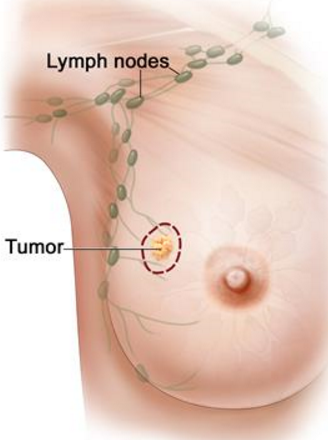
\includegraphics[width=0.3\textwidth]{Booby.png}
\caption{Lymph nodes}
\label{LymphNode}
\end{figure}

\subsubsection*{Data}
The data in this challenge contains a total of 400 whole-slide images (WSIs) of sentinel lymph node from two independent datasets collected in Radboud University Medical Center (Nijmegen, the Netherlands), and the University Medical Center Utrecht (Utrecht, the Netherlands). The training dataset consists of 270 WSIs of lymph node (160 Normal and 110 containing metastases). WSI are generally stored in a multi-resolution pyramid structure. WSI contain multiple downsampled versions of the original image. Each image in the pyramid is stored as a series of tiles, this file structure facilitates rapid retrieval of subregions of the image at different scales as one could not even fit in RAM the tile at the highest resolution, see figure \ref{fig: Pyramid}. These compression technics are similar to those used by Google Earth and they even use the same compression format, jpeg2000. Uncompressed, one image can reach up to 65 GB, the WSI have, at the highest resolution, a size of 96256 x 218624 pixels and have only 188 x 427 pixels at the lowest resolution.


\begin{figure}[!ht]
\centering
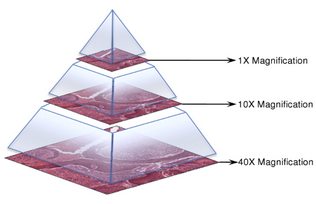
\includegraphics[width=0.5\textwidth]{pyramid.png}
\caption{Pyramid data Structure}
\textit{Between 8 and 10 different resolutions}
\label{fig: Pyramid}
\end{figure}


\subsection{Classification problem}
There was two evaluations and therefore two distinct scoreboards for this challenge. The first is slide based and can be seen as a binary classification, given a Whole-slide Images (WSI) we had to give a confidence score that this WSI contained metastases. The final score for this evaluation was given by the area under the curve (or ROC curve) asserted over 130 test slides. The second was a lesion-based evaluation, this evaluation was aimed to asses the metastases detection within a given slide. This within slide evaluation was measured via a free-response receiver operating characteristic (FROC). This is similar to ROC curve analysis, except that the false positive rate on the x-axis is replaced by the average number of false positives per image. For this challenge, our detection will be considered a true positive, if it falls within an annotated ground truth lesion. The FROC curve is defined as the plot of sensitivity versus the average number of false-positives per image. 

Due to limited time, we tackled these two evaluations as a pixel classification problem in a supervised setting. However for the rest of this paper, I have omitted the second evaluation as we did not correctly perform the pre processing step. Each pixel is described by a vector of features $x \in \mathbb{R}^P$. The training set is composed of a set of such vectors $x^T$,combined in the data matrix $X \in \mathbb{R}^{N \times P}$ and the corresponding labels $Y \in \{0,1\}^N$, provided by the challenge annotators. 
%The concatenation of all vectors is denoted by $X \in
The computational steps and design choices that had to be made can be categorized as follows: 
\begin{enumerate}
	\item Pre-processing of the stained whole-slide images.
	% Feature  extraction. Here, we used a pannel of color and texture
    %     descriptors, evaluated on superpixel regions.
	%\item Sampling strategies in order to derive a reasonably
    %      sized training data set. 
         \item Classification method: here we tested and adapted
           Random Forests and Support Vector Machines. 
         \item Post-processing of the probability map.
\end{enumerate}
%%---------------------------------------
%%---------------------------------------

%\begin{figure}[!ht]
%\centering
%
\includegraphics[width=\textwidth]{Camelyon16.png}
%\caption{Official logo}
%\label{Ol}
%\end{figure}
\subsection{Work pipeline}
Some of the decisions made in this section where a necessity due to the technological difficulties caused by the type of data. In figure \ref{PipelineCam}, I expose a graphic summarising the pre-processing step to the classification problem. The post-processing step is not included in this graphic.

\begin{figure}[!ht]
\centering
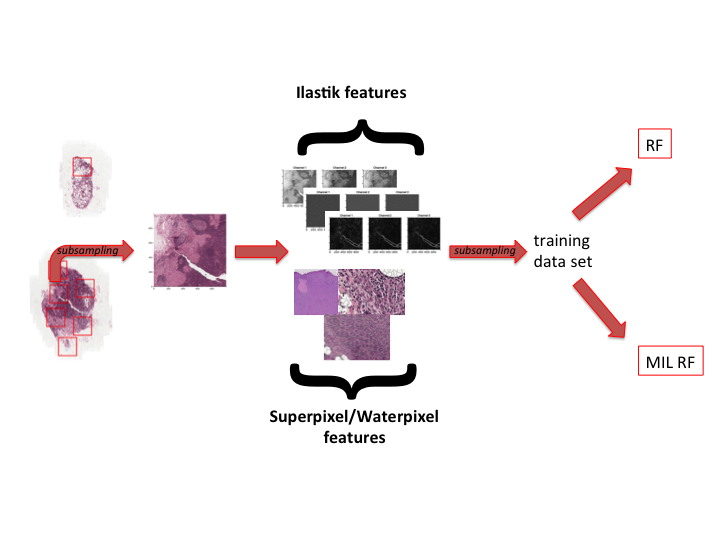
\includegraphics[width=\textwidth]{workflow.png}
\caption{Work pipeline for the Camelyon2016 project.}
\label{PipelineCam}
\end{figure}


\subsubsection*{Pre-processing}

In order to access relevant information in such a tiff file, we had to think carefully as how to segment the whole image to have relevant patches, these patches were a necessity to process the information contained in the slide (Memory constraints). As a WSI is mostly composed of white, processing only the patches containing tissue is used. We applied a threshold segmentation of the WSI at a low resolution, taking the image at a low resolution allowed us to cover the whole image. Once the region of interest were found, we extracted small patches at a very high resolution (resolution number 2) randomly from the WSI. 300 to 400 images of size 1000 x 1000 were extracted per WSI on average. We then applied color deconvolution \citep{deconvolution} to the smaller images in order to obtain a physicologically relevant representation
of the color information. This was done in order to reduce the
computational burden for the subsequent steps.
%A set of 100 \textit{Superpixel-Adaptive Features} (SAF) were used to
%describe each pixel of the train and test image databases. As
%presented in \cite{saf}, these features are well suited for
%segmentation purposes as they are computed on superpixels, i.e. on a
%\textit{computational support} which adapts to the image
%content. 
%Here, we used \textit{waterpixels} \cite{waterpixels}, as they feature
%good adherence to real object boundaries and they are very fast to
%compute. In particular, this allowed us to calculate several
%superpixel partitions, therefore capturing information at different
%scales. 

On each image, we calculated a large panel of different features describing color
and texture of the images. For this, different operators were applied
on the images: identity; a set of operators from Mathematical
Morphology: erosion, opening, top hat and morphological gradient (different
sizes of structuring elements with V6 neighborhood); Haralick texture
features (averaged on all directions). We also applied a family of features based
on Gaussians: difference of gaussians (faster approximation of the
laplacian), eigenvalues of the structure tensor, eigenvalues of
hessian of gaussian based, this family of features are the same set found in the software Ilastik, \url{http://www.ilastik.org/} \citep{Ilastik}.

We evaluated these features on superpixel regions: we first calculated
a partition of the image into superpixels. Here, we used
\textit{waterpixels} \citep{waterpixels}, as they feature good
adherence to real object boundaries and they are very fast to
compute.  In particular, this allowed us to calculate several
superpixel partitions with different size parameters, therefore capturing
information at different scales. The features were then evaluated on
the superpixel regions (average values) at the different
scales. Altogether, we obtained 100 features for each pixel in this step. 

%The partition into waterpixels (with a given set of parameters values)
%was computed once and each pixel was assigned
%the average pixel value within the superpixel it belonged to. 
%
%In order to
%capture multiscale information, we repeated the process with
%waterpixels of different sizes ($step \in \left[ 15,20, 30\right]
%pixels$).\\ 
%
%%---------------------------------------
%%---------------------------------------
\subsubsection*{Classification model}
%%---------------------------------------
%%---------------------------------------
We investigated two classification methods: Random Forests and Support
Vector Machines with RBF kernels. The particularity of the
classification task was an extremely large number of samples ($N \sim  10^{10}$).
Consequently, we could not simply apply the learning algorithms on the
entire data set.  
\begin{enumerate}
\item {\it Random Forests (RF):} Having access to a very large number of
  samples allows us to modify the standard RF procedure. Random
  forests work best, if the individual trees are different from each
  other and cover ``different aspects'' of the data. This is normally
  achieved by boosting, and by randomly drawing the features to be
  considered. With the amount of annotated data we have here, we can
  afford presenting different data to each tree. We therefore generate
  different (but stratified) training sets for each tree of the Random
  Forest.  
\item {\it Support Vector Machines (SVM):} Training with large number
  of samples is generally problematic for non-linear SVM. We therefore
  downsampled the data presented to the classifier. In order to
  properly sample the feature space, we designed a hierarchical
  strategy, where we first apply k-means to each slide, and keep only
  a few representing data points for each cluster. This allowed us
  then to learn an SVM with and RBF kernel. 
\end{enumerate}

Once we have a trained classifier, this allowed us to predict several WSI (via down-sampling) in order to obtain probability maps corresponding to pixel based confidence map of each pixel belonging to a metastasis. Given the results on the cross-validation we choose a Random Forest model as it outperformed on the F1-score. Also, after visual inspection of the probability maps, we thought that the maps produced by the random forest were a lot less noisy than the ones acquired by the Support Vector Machine. The results and parameter tuning are given in table \ref{Cross_val: RF}. We can also take a look at \ref{ProbabilityMapLocalMaxima} which is the output given by our algorithm for the test WSI number 2.

\subsubsection*{Post-processing}

Once we have the probability map of a WSI at a lower resolution we have to decide how to extract the information to better suit the two different tasks, in this report we will describe the procedure for the slide base evaluation. As we choose a RF model, we could take as confidence score of the WSI containing metastasis the maximum value of the probability map. 
%On the other hand, for the lesion-based evaluation, it was difficult as we had to detect each distinct metastasis, but also miss as little as possible. We proceeded as the following: we smoothed the image by applying a gaussian filter followed by an extraction of a local maxima within a connected component as to to reduce this connected region to a single data point.
We can take a look at figure \ref{Detecting maxima} as an example of our metastasis location within a WSI.

\begin{figure}[!ht]
\centering
\begin{subfigure}{.33\textwidth}
  \centering
  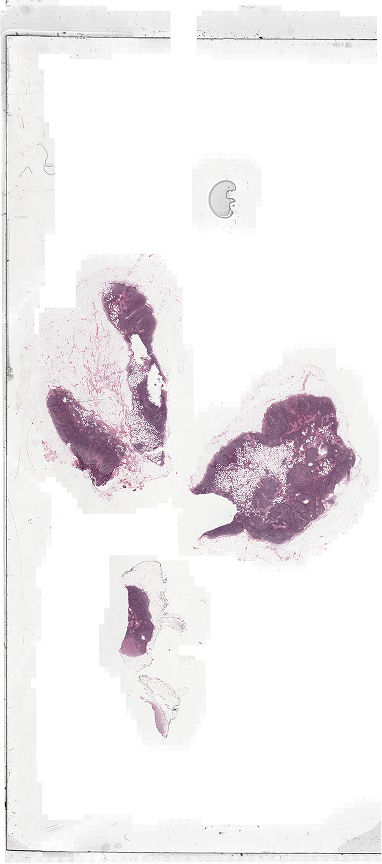
\includegraphics[width=\linewidth]{Test_002_whole.png}
  \caption{RGB raw data.}
  \label{fig:sub1}
\end{subfigure}%
\begin{subfigure}{.33\textwidth}
  \centering
  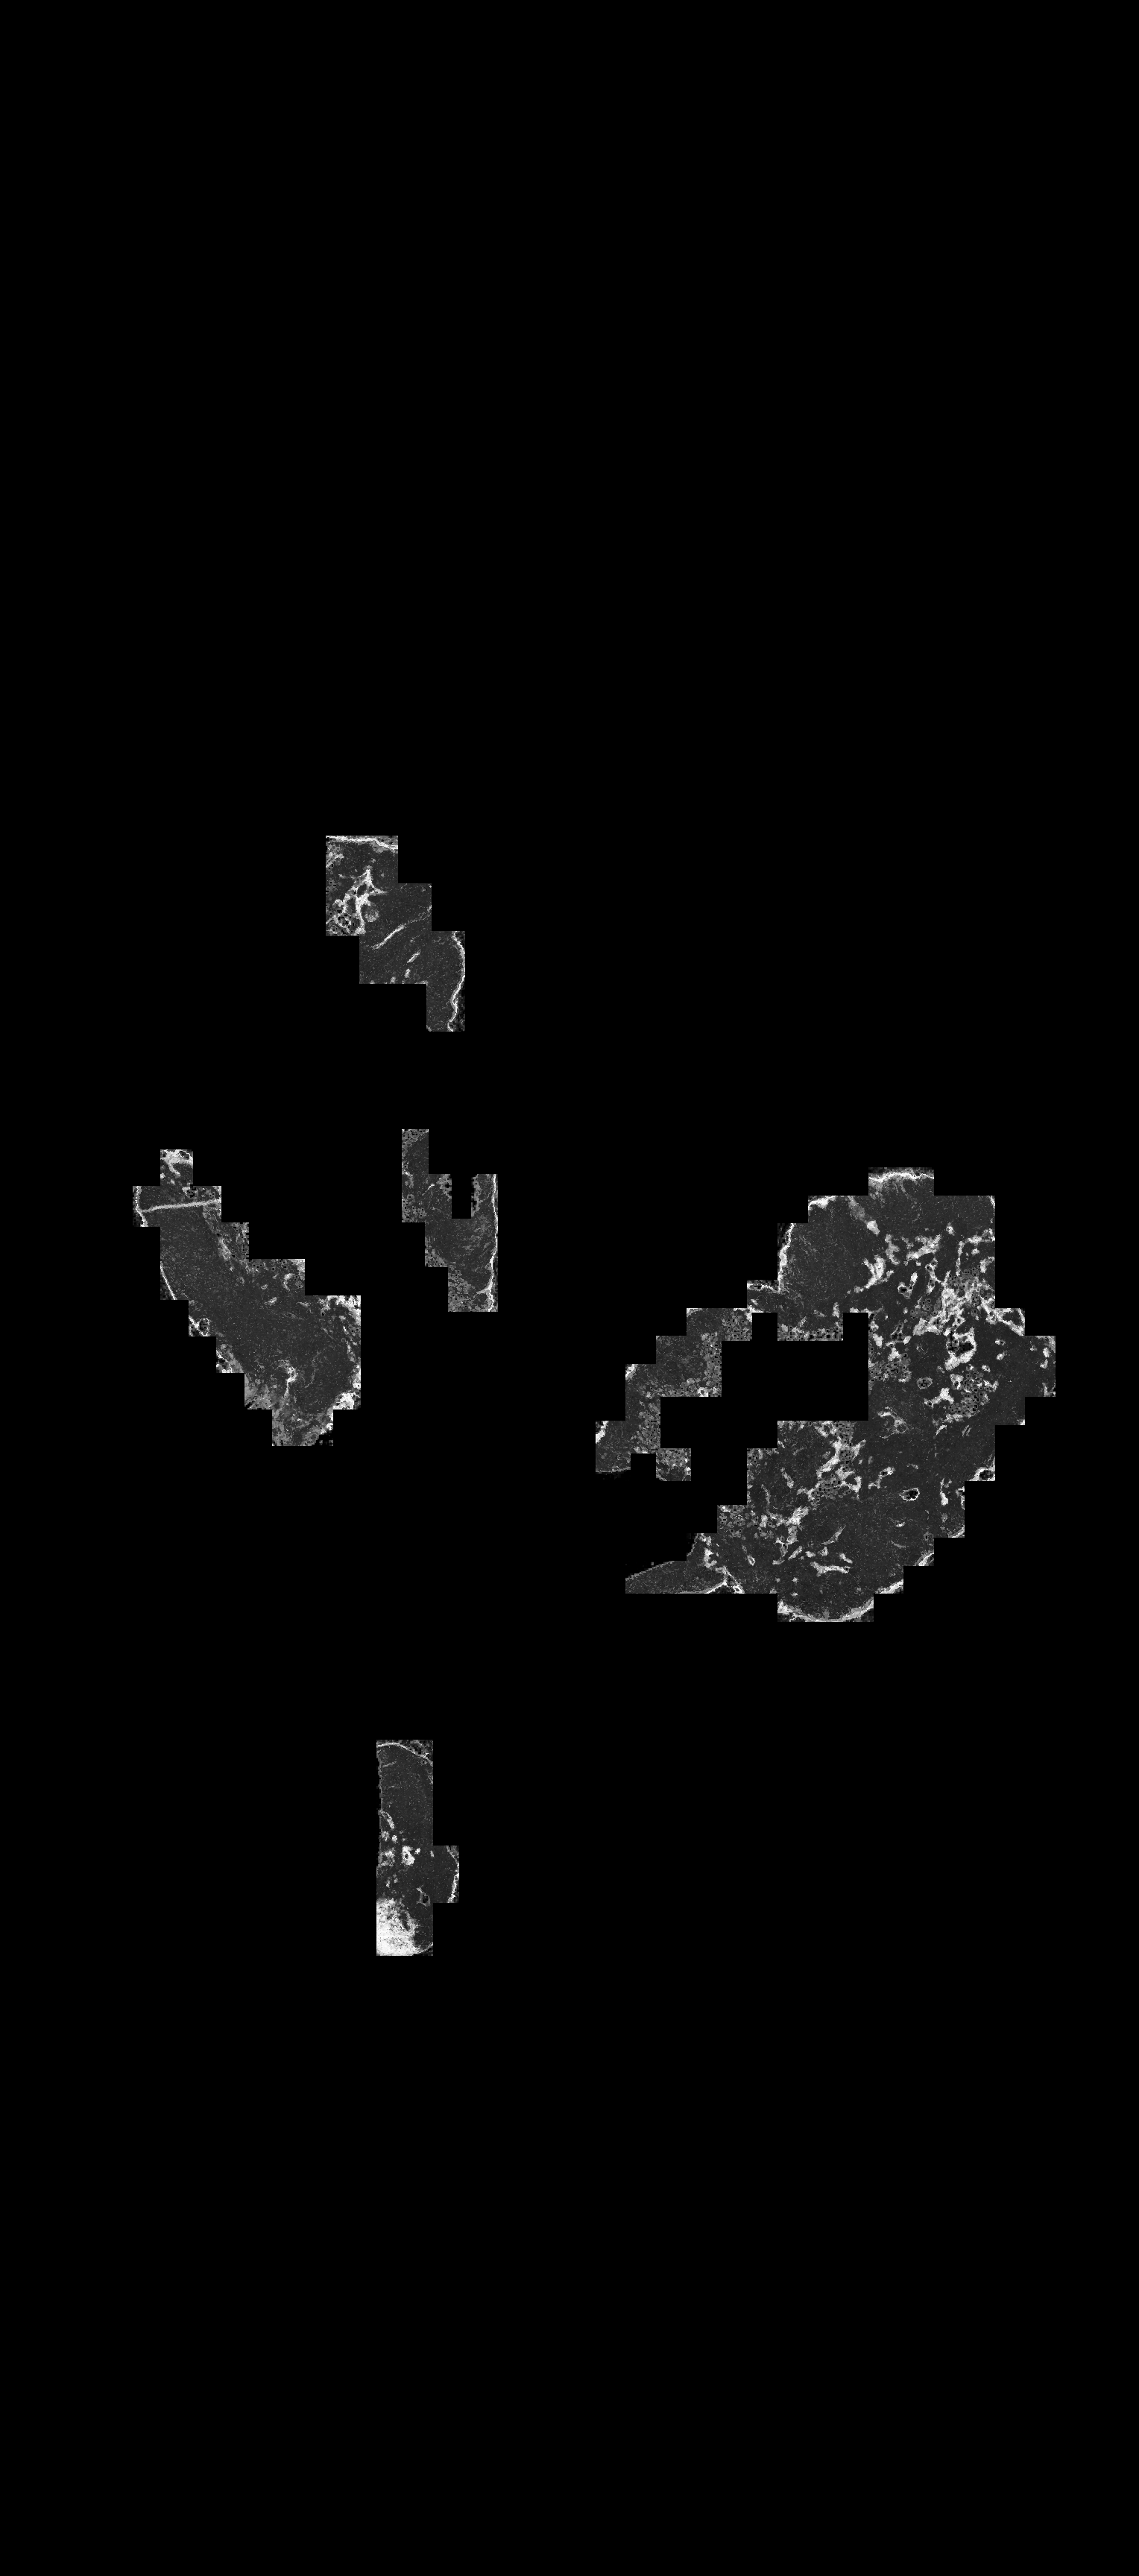
\includegraphics[width=\linewidth]{whole_probmap_Test_002.png}
  \caption{Probability map.}
  \label{ProbabilityMapLocalMaxima}
\end{subfigure}
\begin{subfigure}{.33\textwidth}
  \centering
  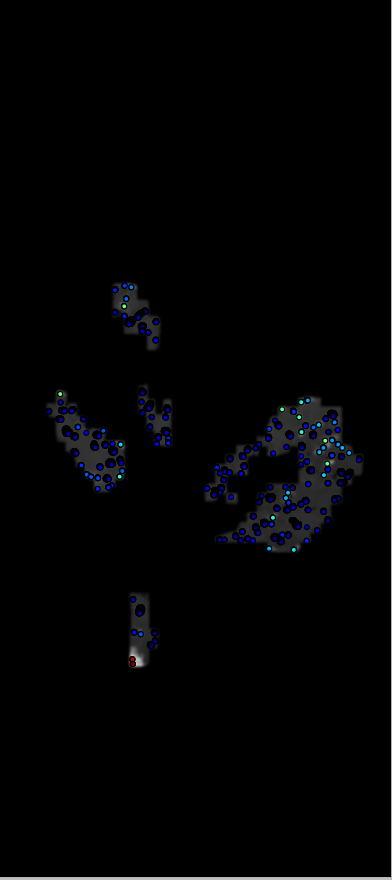
\includegraphics[width=\linewidth]{Detection.png}
  \caption{Metastasis confidence pin-points.}
  \label{Detecting maxima}
\end{subfigure}
\textit{For figure (c), blue is equal to a low confidence score whereas red means a high confidence.}
\caption{Evaluation whole slide image, test slide number 2.}
\label{fig:test}
\end{figure}

\subsubsection*{Different alternative}

We presented our method for the slide-base evaluation, which consists of a pixel classification followed by a pre-processing step. We can by-pass the the pixel classification and the pre-processing by applying a different statistical model. Multiple Instance Learning (MIL) are very well suited in for this slide base evaluation. 
In our case, MIL models will enable use to predict at the slide level with information at a pixel level. On the contrary to standard supervised learning, the algorithm receives a set of labelled bags instead of a set labelled instances. A bag is considered positive if and only if he contains at least one positive In our setting, each bag represents a slide and each instance is a pixel of this slide, for more details see \citep{maron1998multiple}. In pratice, the learning algorithms do not differ in their primal idea, for example a MIL SVM can be formulated as a soft-margin SVM with a extra constraint on the labelled bags: $\sum \frac{y_i+1}{2} \geqslant 1, \forall I \ s.t \ Y_I=1 \ \text{and} \ y_i=-1, \forall I \ s.t \ Y_I=-1$ where $y_i$ is the pixel label, $Y_I$ denotes the bag label and can denote or the label of bag $I$ or the set of pixel inside bag $I$, for more details \citep{andrews2002support}. Random forest can also be adapted to work in MIL framework \citep{leistner2010miforests}. However, due to lack of time we were not able to compare a MIL approach to a our pixel wise classification scheme.



\subsubsection*{Technological difficulties}

Due to the very large size of each WSI, we encountered several difficulties due to data transfer. We have at our disposal 2 clusters, the cluster at Fontainebleau and the one in Curie. This was my first experience using a cluster with a non high-level language. I used the cluster put at disposal by Les Mines at Fontainebleau. This cluster has 424 nodes with several machines of different capacities. However one issue seriously troubled us and slowed us down all along the way as we only understood it close to the deadline, the data transfer speed on our cluster is very low, therefore transferring terabytes of data was very slow. This computation limitation enforced us to have fewer features, experiences and tests. Another issue also related to data transfer, concerns the evaluation scheme with respect to the tuning of each model, we couldn't use the same metric as the one given by the challenge as this one implies predicting over a WSI. This was not possible in terms of time and of computation, instead we had to maximize over the F1-score, see table \ref{Cross_val: RF} for the results for the random forest and table \ref{Cross_val: SVM} for those with the SVM with the RBF kernel.

Another difficulty was opening the data files, we used the OpenSlide library that is written in C++.
This challenge was very rewarding as the he taught me a huge amount about cluster policies, organisation and use!


\subsection{Challenge Results and ISBI 2016}

As I participated to this challenge it was interesting for me to attend the presentations concerning it. We were among the 23 teams out of the 208 teams that submitted a solution. We obtained an Area Under the Curve of 0.63 and obtained a final ranking 22nd, see figure \ref{Eval: ROC}. Of the 23 submissions, only 3 used "classical methods" (on the contrary to neural networks) to extract information from the WSI. The best of these three teams reached an area under the ROC curve of 0.76 and finished 11. The 3rd team performing classical methods was last. After a brief presentation of the best performing team within classical extraction method, we would hope that our method could reach 0.76 via a better tuning, with respect to the feature, model parameters and model evaluation. Indeed, they had the same pipeline with the same main parts as ours. However, all the other teams used pre-trained or existing architecture and achieved much better result than the classical methods. This gave us a clear view of my next interest, deep neural networks.

\begin{figure}[!ht]
\centering
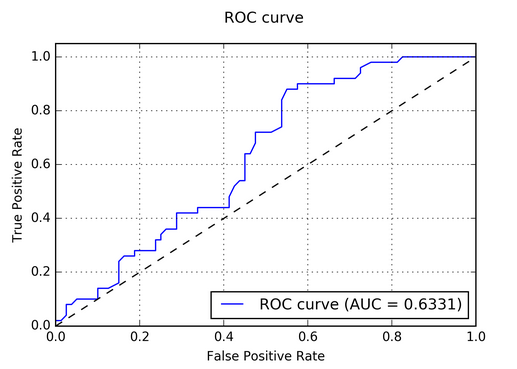
\includegraphics[width=0.5\textwidth]{ROC.png}
\caption{ROC curve associated to the slide base evaluation}
\label{Eval: ROC}
\end{figure}

This challenge might have been a bit early for me to be truly competitive. Some of the finalist, were advanced labs that tackle on a daily bases segmentation problems. This was my very first experience dealing with histopathology data, mathematical morphology, cluster of computers and team work among different labs. 

The conference was held in Prague and I also attended a tutorial on deep neural networks that was given at the end. It lasted 4 days and to the surprise of some, histopathology has gained in popularity as you could easily end up listening to only histopathology talks. In most histopathology talks, neural network, the state of the art in image processing were used. It seems, as I focus on application, that it is essential for me to try and to apply deep convolutionnal network.


\section{May 2016 and future work}
From May to now, my main focus has returned to the datasets provided by the collaborations involved in this PhD. In particular I had to acquire the data set from F. Reyal. The work pipeline for this project is pictured in \ref{workflow1}. The pipeline can be divided in three parts: computer vision in order to extract encoded information from the raw images. The second is feature extraction on two levels, the biological image data driven features and the extraction of the other data type. This data type can be molecular driven, transcriptomic, another type of image data. The final part of this project will then be to derive a statistical model in order to find correlations between the different types of data, improve prognosis prediction and overall try to better quantify and understand cancer progression. I will only discuss part one as it is the one I am currently at.

\begin{figure}[!ht]
\centering
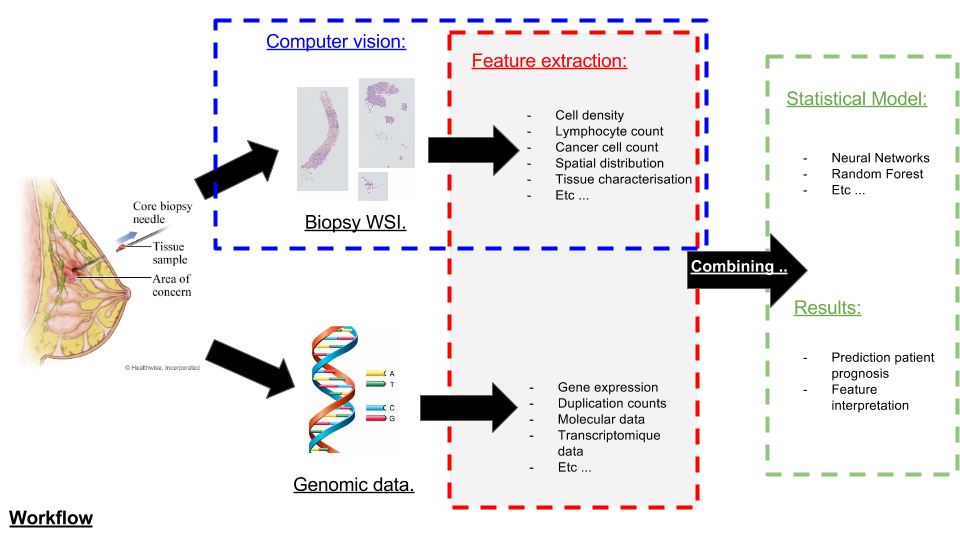
\includegraphics[width=\textwidth]{Workflow.png}
\caption{Workflow}
\label{workflow1}
\end{figure}


\subsection{Data}

The tissue samples were extracted from the patients in two steps, first was performed a biopsy extraction as it is pictured in \ref{workflow1}, a biopsy sample is a thin piece of tissue that can be performed without a full surgery. A biopsy will inform the practitioner if he must perform surgery to remove the tumor or apply a chemotherapy based treatment. Here however, all patients received a chemotherapy based treatment after the biopsy. After the treatment, in order to asses the progression of the cancer, the surgeons extracted whole tumor slides from the patients. We also have genomic, clinical data for some patients, but this part will not be discussed as it has not been dealt with yet. Having this data scheme could allow us to extract more information on top of the primal objective, in particular we could try and quantify patients response to chemotherapy.

\subsection{Computer vision}

The detailed pipeline for this part can be seen in \ref{ComputerVision}, this scheme is similar in the first steps to those performed in the camelyon challenge 2016. In this first steps, we wish to find regions of interest, which can be resumed to finding the tissue areas in the WSI. The data here was a lot more messier, some annotations were performed via a permanent marker on several slides and had to be removed. The slide label was also in most of the WSI and had to be removed via a pixel value segmentation. Once the tissue information was discovered in the WSI, we extracted small patches of size 512 x 512.

We wish to create biological features with the help of the pathologist. Similar to the work done in \citet{yuan2012quantitative}, we wish to have revelant features. They extract valuable information including: Lymphocytes counts, stromal count, cancer cell count, WSI density profiles, mitotic density counts and so on. However in order to create this biological driven features we have to properly segment the histopathology data. Due to the recent advances in deep neural networks and lately for their performances in segmentation and in medical imaging \citep{UNet,long2015fcn} I wished to become more familiar. I familiarized myself with GPU hardware and with the caffe librabry: \url{http://caffe.berkeleyvision.org/} \citep{jia2014caffe}. Good hardware becomes a necessity when training deep network as it can increase the computation time by x50. The Center for computational biology has a GEFORCE GTX TITAN Z NVIDIA graphics card and I am still struggling to find a suitable place to power it.
Once the GPU installed, I will be able to fine tune a Fully Convolutionnal Network (FCN) for semantic segmentation \citep{long2015fcn}. On a different note, we will need annotated data for this segmentation task. I will therefore be providing pathologist with a software to enable them to create manual segmentation of the image, via the ITK-SNAP toolkit: \url{www.itksnap.org} \citep{py06nimg}. An issue with creating our own ground-truth is related to the tediousness and yet complicated manual task of segmentation. In one image, you can find up to 50 or 60 cells, so it can be a very long procedure and we can't ask a single pathologist to annotate more then 20 images. To counter balance this lack in data, which is crucial with respect to the training in deep networks, we will augment the data set as described in \citet{UNet} by manual flipping, rotating, creating out of focus effect and by doing elastic transformations of the image. Data augmentation is an important step for the training as it is thanks to these multiple transformations that our model will learn the appropriate invariances,  see section 5.5 in \citep{bishop2006pattern}. We augment the data by shift, \ref{fig:shift}, by rotation, \ref{fig:rot}, by flipping it, \ref{fig:flip} and by doing elastic distortions, \ref{fig:elastic}. Creating out of focus images to augment the data can also be used to learn invariances corresponding to errors caused by the scanner being out of focus, see figure \ref{fig:blur}. This is done by convolving the image with a normalized box filter. In \ref{fig:blur} we used a box filter of size 10. 


\begin{figure}[!ht]
\centering
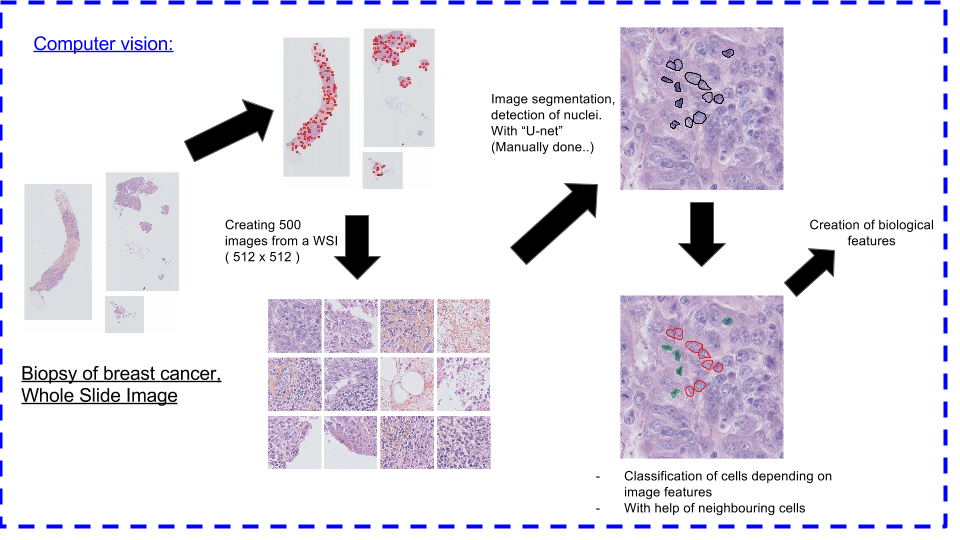
\includegraphics[width=\textwidth]{ComputerVision.png}
\caption{Computer Vision aspect}
\label{ComputerVision}
\end{figure}

\begin{figure}
\begin{multicols}{3}
	\begin{subfigure}{0.3\textwidth}
    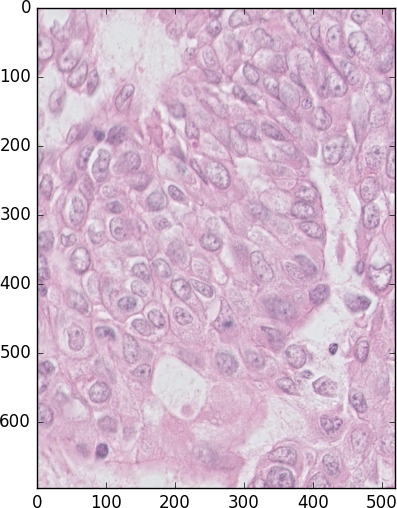
\includegraphics[width=0.9\textwidth]{BIS.png}\par 
     \caption{Original image}
     \label{fig:original}
	\end{subfigure}%
	\begin{subfigure}{0.3\textwidth}
    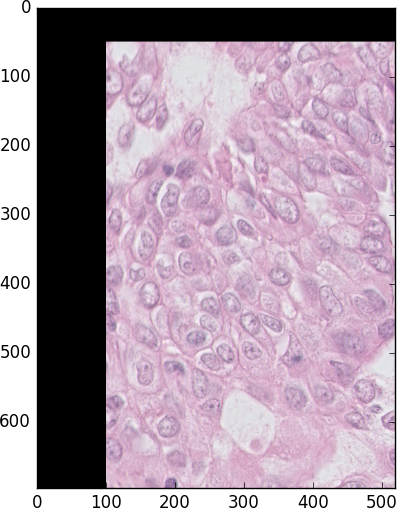
\includegraphics[width=0.9\textwidth]{shift.png}\par 
    \caption{Translated}
    \label{fig:shift}
	\end{subfigure}%
	\begin{subfigure}{0.3\textwidth}
    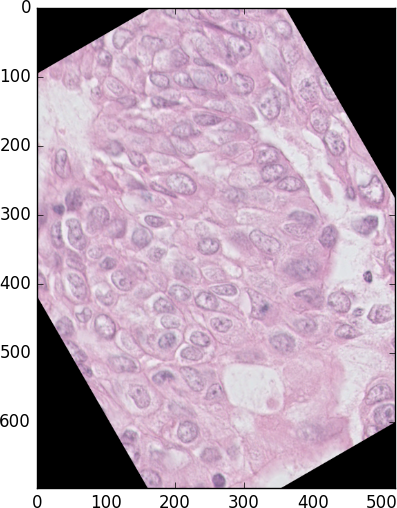
\includegraphics[width=0.9\textwidth]{rot.png}\par 
     \caption{Rotated}
     \label{fig:rot}
	\end{subfigure}%
\end{multicols}
\begin{multicols}{3}

    \begin{subfigure}{0.3\textwidth}
    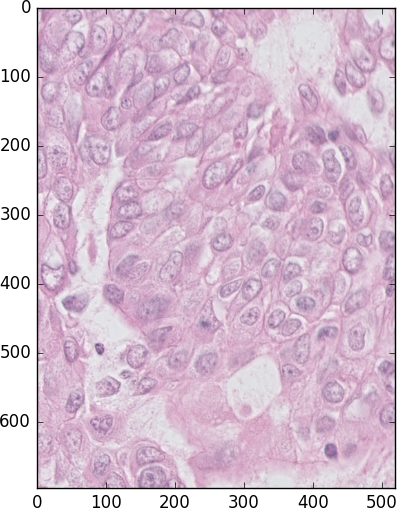
\includegraphics[width=0.9\textwidth]{flip.png}\par 
     \caption{Vertical flip}
     \label{fig:flip}
	\end{subfigure}%
	\begin{subfigure}{0.3\textwidth}
    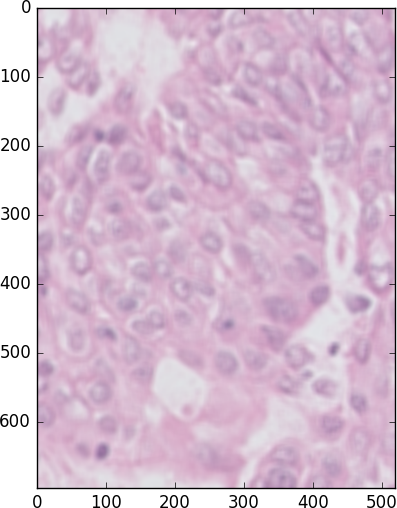
\includegraphics[width=0.9\textwidth]{blur.png}\par 
    \caption{Out of focus}
    \label{fig:blur}
	\end{subfigure}%
	\begin{subfigure}{0.3\textwidth}
    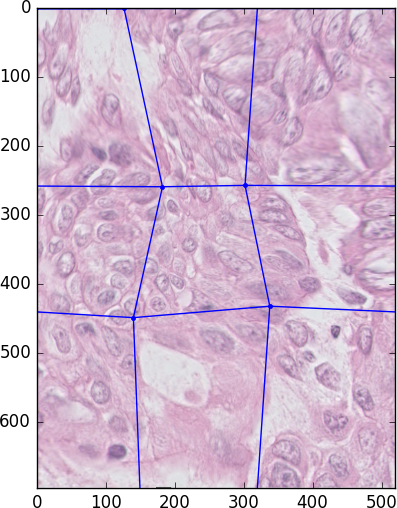
\includegraphics[width=0.9\textwidth]{ELAST.png}\par 
     \caption{Elastic deformation}
     \label{fig:elastic}
	\end{subfigure}%
\end{multicols}
\caption{Data augmentation}
\end{figure}

\section{Additionnal notes}

During this first year I attended two courses focused on image processing, the first was in mathematical morphology and is taught by members of the Centre for Mathematical Morphology. It was organized as an intense week course. Furthermore I attended the course \textit{Object recognition and computer vision} proposed by ENS Cachan. 
I will also be attending the machine learning summer school (MLSS) organized this year in Peru.

%\begin{figure}[!ht]
%\centering
%\includegraphics[width=\textwidth]{}
%\caption{}
%\label{}
%\end{figure}

\section{Futur Work}

Collecting annotated data for segmentation is the next step. To help annotate, we will initialize the manual segmentation thanks to previous work. This work, based on mathematical morphology, segments nucleus in the given picture In order to have \textit{true} annotated ground truth about the segmentation, we will manually correct the segmentation output of the mathematical morphology based segmentation. Succeeding in training a fully convolutionnal will be the next step closely followed by the final two parts of the pipeline, i.e. biological feature extraction and elaboration of the statistical model. 

\newpage
\section*{Appendix: cross-validation results}

\begin{table}[!ht]

\centering
\begin{footnotesize}
\begin{tabular}{llllrrrr}
\toprule
 n\_tree    &  m\_try  & n\_bootstrap     &  n\_subsampling    &  Precision &     Recall &         F1 &   Accuracy \\
\midrule
1000 & 10 & 1000 & 2000 &            &            &            &            \\
     & 15 &      &      &       0.87 &       0.22 &       0.35 &       0.86 \\
     &    & 2000 &      &       0.86 &       0.20 &       0.32 &       0.85 \\
     & 20 & 1000 &      &       0.88 &       0.23 &       0.36 &       0.85 \\
     &    & 5000 &      &       0.64 &       0.12 &       0.20 &       0.84 \\
     & 30 & 2000 &      &       0.64 &       0.13 &       0.22 &       0.86 \\
     & 50 & 500 &      &       0.92 &       0.22 &       0.36 &       0.87 \\
     &    & 5000 &      &       0.88 &       0.22 &       0.35 &       0.85 \\
\textcolor{red}{500} & 10 & 1000 &      &       0.75 &       0.17 &       0.28 &       0.86 \\
     &    &      & 5000 &       0.82 &       0.08 &       0.14 &       0.84 \\
     &    & 10000 & 2000 &       0.69 &       0.02 &       0.03 &       0.84 \\
     &    &      & 5000 &       0.83 &       0.10 &       0.17 &       0.88 \\
     &    & 2000 & 2000 &       0.81 &       0.04 &       0.08 &       0.90 \\
     &    &      & 5000 &       0.88 &       0.28 &       0.40 &       0.85 \\
     &    & 500 & 2000 &       0.71 &       0.02 &       0.04 &       0.85 \\
     &    & 5000 &      &       0.85 &       0.23 &       0.33 &       0.84 \\
     &    &      & 5000 &       0.81 &       0.14 &       0.21 &       0.87 \\
     & 15 & 1000 & 2000 &       0.82 &       0.02 &       0.04 &       0.87 \\
     &    &      & 5000 &       0.85 &       0.31 &       0.43 &       0.84 \\
     &    & 10000 & 2000 &       0.95 &       0.05 &       0.10 &       0.83 \\
     &    &      & 5000 &       0.90 &       0.09 &       0.17 &       0.88 \\
     &    & 2000 & 2000 &       0.76 &       0.03 &       0.06 &       0.90 \\
     &    &      & 5000 &       0.85 &       0.14 &       0.22 &       0.85 \\
     &    & 500 & 2000 &       0.87 &       0.04 &       0.08 &       0.86 \\
     &    &      & 5000 &       0.89 &       0.12 &       0.20 &       0.84 \\
     &    & 5000 & 2000 &       0.83 &       0.03 &       0.06 &       0.83 \\
     &    &      & 5000 &       0.84 &       0.15 &       0.24 &       0.87 \\
     & \textcolor{red}{20} & \textcolor{red}{1000} & 2000 &       0.84 &       0.03 &       0.05 &       0.88 \\
     &    &      & \textcolor{red}{5000} &       \textcolor{red}{0.86} &       \textcolor{red}{0.33} &       \textcolor{red}{0.45} &       \textcolor{red}{0.84} \\
     &    & 10000 & 2000 &       0.84 &       0.04 &       0.08 &       0.86 \\
     &    &      & 5000 &       0.88 &       0.13 &       0.23 &       0.89 \\
     &    & 2000 & 2000 &       0.85 &       0.04 &       0.08 &       0.90 \\
     &    &      & 5000 &       0.88 &       0.13 &       0.21 &       0.86 \\
     &    & 500 & 2000 &       0.91 &       0.04 &       0.08 &       0.85 \\
     &    &      & 5000 &       0.90 &       0.21 &       0.32 &       0.85 \\
     &    & 5000 & 2000 &       0.94 &       0.05 &       0.09 &       0.82 \\
     &    &      & 5000 &       0.80 &       0.24 &       0.34 &       0.86 \\
     & 30 & 1000 & 2000 &       0.76 &       0.03 &       0.05 &       0.89 \\
     &    &      & 5000 &       0.88 &       0.14 &       0.22 &       0.85 \\
     &    & 10000 & 2000 &       0.82 &       0.03 &       0.06 &       0.86 \\
     &    &      & 5000 &       0.84 &       0.10 &       0.17 &       0.89 \\
     &    & 2000 & 2000 &       0.86 &       0.03 &       0.06 &       0.89 \\
     &    &      & 5000 &       0.87 &       0.12 &       0.20 &       0.86 \\
     &    & 500 & 2000 &       0.91 &       0.07 &       0.13 &       0.88 \\
     &    &      & 5000 &       0.89 &       0.18 &       0.29 &       0.83 \\
     &    & 5000 & 2000 &       0.91 &       0.09 &       0.16 &       0.88 \\
     &    &      & 5000 &       0.83 &       0.15 &       0.23 &       0.87 \\
     & 50 & 1000 & 2000 &       0.82 &       0.04 &       0.07 &       0.89 \\
     &    &      & 5000 &       0.90 &       0.12 &       0.20 &       0.85 \\
     &    & 10000 & 2000 &       0.87 &       0.06 &       0.10 &       0.86 \\
     &    &      & 5000 &       0.82 &       0.11 &       0.18 &       0.89 \\
     &    & 2000 & 2000 &       0.77 &       0.03 &       0.06 &       0.90 \\
     &    &      & 5000 &       0.88 &       0.18 &       0.27 &       0.86 \\
     &    & 500 & 2000 &       0.81 &       0.06 &       0.10 &       0.88 \\
     &    & 5000 &      &       0.88 &       0.24 &       0.35 &       0.82 \\
     &    &      & 5000 &       0.82 &       0.19 &       0.28 &       0.87 \\
\bottomrule

\end{tabular}
\end{footnotesize}
\caption{Performance estimated for our type of random forests by cross validation (10-fold)}
\label{Cross_val: RF}
\end{table}

\newpage

\newgeometry{left=2.3cm,bottom=0.5cm,right=-1cm}

\begin{table}[!ht]
\begin{multicols}{2}
\centering
\begin{scriptsize}
\begin{tabular}{|lllrrrr|}
\toprule
   c   &   gamma    &  n\_samples   &  Precision &     Recall &         F1 &   Accuracy \\
\midrule
0.001 & 0.001 & 10000 &            &            &            &            \\
      &       & 2000 &       1.00 &       0.10 &       0.18 &       0.10 \\
      &       & 5000 &       1.00 &       0.11 &       0.20 &       0.12 \\
      & 0.01 & 10000 &       1.00 &       0.11 &       0.20 &       0.11 \\
      &       & 2000 &       0.92 &       0.17 &       0.29 &       0.49 \\
      &       & 5000 &       0.85 &       0.21 &       0.33 &       0.56 \\
      & 0.1 & 10000 &       0.90 &       0.18 &       0.29 &       0.50 \\
      &       & 2000 &       1.00 &       0.12 &       0.21 &       0.12 \\
      &       & 5000 &       0.83 &       0.15 &       0.22 &       0.29 \\
      & 1 & 10000 &       1.00 &       0.11 &       0.21 &       0.11 \\
      &       & 2000 &       1.00 &       0.12 &       0.22 &       0.12 \\
      &       & 5000 &       1.00 &       0.11 &       0.19 &       0.11 \\
      & 10 & 10000 &       1.00 &       0.10 &       0.18 &       0.10 \\
      &       & 2000 &       1.00 &       0.12 &       0.22 &       0.12 \\
      &       & 5000 &       1.00 &       0.08 &       0.15 &       0.08 \\
      & 100 & 10000 &       1.00 &       0.11 &       0.20 &       0.11 \\
      &       & 2000 &       1.00 &       0.12 &       0.21 &       0.12 \\
      &       & 5000 &       1.00 &       0.08 &       0.15 &       0.08 \\
      & 1000 & 10000 &       1.00 &       0.11 &       0.21 &       0.11 \\
      &       & 2000 &       1.00 &       0.12 &       0.21 &       0.12 \\
      &       & 5000 &       1.00 &       0.08 &       0.15 &       0.08 \\
      & 	  &		 &            &            &            &            \\
 ...  &  ...  & ...  &   ...      &   ...      &   ...      &   ...      \\
      & 	  &		 &            &            &            &            \\
0.1 & 0.001 & 10000 &       1.00 &       0.11 &       0.20 &       0.11 \\
      &       & 2000 &       0.94 &       0.17 &       0.29 &       0.49 \\
      &       & 5000 &       0.93 &       0.18 &       0.29 &       0.50 \\
      & 0.01 & 10000 &       0.93 &       0.17 &       0.29 &       0.49 \\
      &       & 2000 &       0.82 &       0.23 &       0.36 &       0.68 \\
      &       & 5000 &       0.82 &       0.24 &       0.36 &       0.68 \\
      & 0.1 & 10000 &       0.82 &       0.24 &       0.36 &       0.68 \\
      &       & 2000 &       0.66 &       0.33 &       0.44 &       0.82 \\
      &       & 5000 &       0.62 &       0.32 &       0.42 &       0.81 \\
      & 1 & 10000 &       0.66 &       0.33 &       0.44 &       0.82 \\
      &       & 2000 &       1.00 &       0.12 &       0.21 &       0.12 \\
      &       & 5000 &       0.00 &       0.02 &       0.00 &       0.85 \\
      & 10 & 10000 &       1.00 &       0.10 &       0.18 &       0.10 \\
      &       & 2000 &       1.00 &       0.10 &       0.19 &       0.10 \\
      &       & 5000 &       1.00 &       0.15 &       0.26 &       0.15 \\
      & 100 & 10000 &       1.00 &       0.11 &       0.19 &       0.11 \\
      &       & 2000 &       1.00 &       0.10 &       0.18 &       0.10 \\
      &       & 5000 &       1.00 &       0.15 &       0.26 &       0.15 \\
      & 1000 & 10000 &       1.00 &       0.11 &       0.20 &       0.11 \\
      &       & 2000 &       1.00 &       0.11 &       0.20 &       0.11 \\
      &       & 5000 &       1.00 &       0.15 &       0.26 &       0.15 \\
0.2 & 0.001 & 10000 &       1.00 &       0.10 &       0.17 &       0.10 \\
      &       & 2000 &       0.91 &       0.19 &       0.31 &       0.54 \\
      &       & 5000 &       0.91 &       0.19 &       0.31 &       0.54 \\
      & 0.01 & 10000 &       0.92 &       0.18 &       0.30 &       0.54 \\
      &       & 2000 &       0.81 &       0.24 &       0.37 &       0.69 \\
      &       & 5000 &       0.81 &       0.25 &       0.38 &       0.70 \\
      & 0.1 & 10000 &       0.81 &       0.24 &       0.37 &       0.70 \\
      &       & 2000 &       0.67 &       0.34 &       0.45 &       0.82 \\
      &       & 5000 &       0.67 &       0.34 &       0.45 &       0.82 \\
      & 1 & 10000 &       0.66 &       0.34 &       0.44 &       0.82 \\
      &       & 2000 &       0.02 &       0.58 &       0.05 &       0.89 \\
      &       & 5000 &       0.03 &       0.60 &       0.05 &       0.89 \\
0.5 & 0.001 & 10000 &       0.02 &       0.65 &       0.04 &       0.89 \\
      &       & 2000 &       0.90 &       0.20 &       0.32 &       0.58 \\
      &       & 5000 &       0.90 &       0.20 &       0.32 &       0.58 \\
      & 0.01 & 10000 &       0.89 &       0.20 &       0.32 &       0.58 \\
      &       & 2000 &       0.78 &       0.26 &       0.39 &       0.73 \\
      &       & 5000 &       0.79 &       0.27 &       0.39 &       0.73 \\
      & 0.1 & 10000 &       0.78 &       0.26 &       0.39 &       0.73 \\
      &       & 2000 &       0.63 &       0.37 &       0.46 &       0.85 \\
      &       & 5000 &       0.63 &       0.37 &       0.46 &       0.85 \\
      & 1 & 10000 &       0.64 &       0.38 &       0.47 &       0.85 \\
      &       & 2000 &       0.00 &       0.79 &       0.00 &       0.88 \\
      &       & 5000 &       0.00 &       0.93 &       0.00 &       0.88 \\
1 & 0.001 & 10000 &       0.00 &       0.87 &       0.00 &       0.88 \\
      &       & 2000 &       0.89 &       0.20 &       0.33 &       0.60 \\
      &       & 5000 &       0.89 &       0.21 &       0.33 &       0.60 \\
      & 0.01 & 10000 &       0.89 &       0.20 &       0.33 &       0.60 \\
      &       & 2000 &       0.77 &       0.28 &       0.41 &       0.76 \\
      &       & 5000 &       0.75 &       0.29 &       0.41 &       0.77 \\
      & 0.1 & 10000 &       0.77 &       0.29 &       0.41 &       0.76 \\
      &       & 2000 &       0.58 &       0.42 &       0.48 &       0.87 \\
      &       & 5000 &       0.35 &       0.52 &       0.41 &       0.90 \\
      & 1 & 10000 &       0.58 &       0.42 &       0.48 &       0.87 \\
      &       & 5000 &       0.00 &       0.98 &       0.00 &       0.88 \\
 \bottomrule
\end{tabular}     
\\
\begin{tabular}{|lllrrrr|}
\toprule
   c   &   gamma    &  n\_samples     &  Precision &     Recall &         F1 &   Accuracy \\
\midrule

10 & 0.001 & 10000 &       0.00 &       0.91 &       0.00 &       0.88 \\
      &       & 2000 &       0.83 &       0.23 &       0.36 &       0.68 \\
      &       & 5000 &       0.83 &       0.24 &       0.36 &       0.68 \\
      & 0.01 & 10000 &       0.84 &       0.24 &       0.37 &       0.68 \\
      &       & 2000 &       0.67 &       0.36 &       0.46 &       0.83 \\
      &       & 5000 &       0.55 &       0.37 &       0.44 &       0.85 \\
      & 0.1 & 10000 &       0.67 &       0.36 &       0.47 &       0.84 \\
      &       & 2000 &       0.44 &       0.52 &       0.47 &       0.90 \\
      &       & 5000 &       0.21 &       0.64 &       0.31 &       0.90 \\
      & 1 & 10000 &       0.43 &       0.51 &       0.46 &       0.90 \\
      &       & 5000 &       0.00 &       0.92 &       0.00 &       0.88 \\
100 & 0.001 & 10000 &       0.00 &       0.90 &       0.00 &       0.89 \\
      &       & 2000 &       0.78 &       0.28 &       0.41 &       0.76 \\
      &       & 5000 &       0.75 &       0.26 &       0.39 &       0.75 \\
      & 0.01 & 10000 &       0.77 &       0.28 &       0.41 &       0.76 \\
      &       & 2000 &       0.58 &       0.41 &       0.47 &       0.86 \\
      &       & 5000 &       0.35 &       0.48 &       0.39 &       0.89 \\
      & 0.1 & 10000 &       0.57 &       0.40 &       0.47 &       0.86 \\
      &       & 2000 &       0.43 &       0.51 &       0.46 &       0.90 \\
      &       & 5000 &       0.21 &       0.65 &       0.30 &       0.90 \\
      & 1 & 10000 &       0.44 &       0.51 &       0.46 &       0.90 \\
      &       & 5000 &       0.00 &       0.97 &       0.00 &       0.88 \\
1000 & 0.001 & 10000 &       0.00 &       0.81 &       0.00 &       0.89 \\
      &       & 2000 &       0.70 &       0.33 &       0.45 &       0.81 \\
      &       & 5000 &       0.56 &       0.33 &       0.41 &       0.83 \\
      & 0.01 & 10000 &       0.69 &       0.33 &       0.44 &       0.81 \\
      &       & 2000 &       0.49 &       0.43 &       0.45 &       0.88 \\
      &       & 5000 &       0.27 &       0.49 &       0.34 &       0.89 \\
      & 0.1 & 10000 &       0.49 &       0.43 &       0.46 &       0.88 \\
      &       & 2000 &       0.42 &       0.50 &       0.45 &       0.89 \\
      &       & 5000 &       0.22 &       0.66 &       0.31 &       0.90 \\
      & 1 & 10000 &       0.43 &       0.51 &       0.46 &       0.90 \\
      &       & 5000 &       0.00 &       0.96 &       0.00 &       0.88 \\
\textcolor{red}{2} & 0.001 & 10000 &       0.00 &       0.93 &       0.00 &       0.88 \\
      &       & 2000 &       0.87 &       0.21 &       0.34 &       0.62 \\
      &       & 5000 &       0.88 &       0.21 &       0.34 &       0.63 \\
      & 0.01 & 10000 &       0.87 &       0.21 &       0.34 &       0.63 \\
      &       & 2000 &       0.74 &       0.31 &       0.43 &       0.79 \\
      &       & 5000 &       0.74 &       0.31 &       0.44 &       0.80 \\
      & \textcolor{red}{0.1} & 10000 &       0.74 &       0.31 &       0.43 &       0.79 \\
      &       & 2000 &       0.51 &       0.46 &       0.48 &       0.89 \\
      &       & \textcolor{red}{5000} &       \textcolor{red}{0.52} &       \textcolor{red}{0.47} &       \textcolor{red}{0.49} &        \textcolor{red}{0.89} \\
      & 1 & 10000 &       0.51 &       0.46 &       0.48 &       0.89 \\
      &       & 2000 &       0.00 &       0.97 &       0.00 &       0.88 \\
      &       & 5000 &       0.00 &       0.88 &       0.00 &       0.88 \\
20 & 0.001 & 10000 &       0.00 &       0.99 &       0.00 &       0.88 \\
      &       & 2000 &       0.82 &       0.25 &       0.37 &       0.70 \\
      &       & 5000 &       0.82 &       0.25 &       0.38 &       0.71 \\
      & 0.01 & 10000 &       0.82 &       0.25 &       0.38 &       0.70 \\
      &       & 2000 &       0.64 &       0.37 &       0.47 &       0.84 \\
      &       & 5000 &       0.64 &       0.38 &       0.47 &       0.85 \\
      & 0.1 & 10000 &       0.64 &       0.38 &       0.47 &       0.85 \\
      &       & 2000 &       0.44 &       0.51 &       0.47 &       0.90 \\
      &       & 5000 &       0.43 &       0.52 &       0.46 &       0.90 \\
      & 1 & 10000 &       0.43 &       0.51 &       0.46 &       0.90 \\
      &       & 2000 &       0.00 &       0.94 &       0.00 &       0.88 \\
      &       & 5000 &       0.00 &       0.86 &       0.00 &       0.88 \\
200 & 0.001 & 10000 &       0.00 &       0.99 &       0.00 &       0.88 \\
      &       & 2000 &       0.76 &       0.31 &       0.43 &       0.78 \\
      &       & 5000 &       0.75 &       0.30 &       0.43 &       0.78 \\
      & 0.01 & 10000 &       0.75 &       0.30 &       0.42 &       0.78 \\
      &       & 2000 &       0.54 &       0.42 &       0.47 &       0.87 \\
      &       & 5000 &       0.53 &       0.41 &       0.46 &       0.87 \\
      & 0.1 & 10000 &       0.54 &       0.41 &       0.46 &       0.87 \\
      &       & 2000 &       0.43 &       0.51 &       0.46 &       0.90 \\
      &       & 5000 &       0.44 &       0.51 &       0.47 &       0.90 \\
      & 1 & 10000 &       0.43 &       0.50 &       0.45 &       0.89 \\
      &       & 2000 &       0.00 &       0.86 &       0.00 &       0.88 \\
      &       & 5000 &       0.00 &       0.91 &       0.00 &       0.88 \\
2000 & 0.001 & 10000 &       0.00 &       0.78 &       0.00 &       0.88 \\
      &       & 2000 &       0.66 &       0.34 &       0.45 &       0.82 \\
      &       & 5000 &       0.68 &       0.35 &       0.46 &       0.83 \\
      & 0.01 & 10000 &       0.68 &       0.34 &       0.45 &       0.82 \\
      &       & 2000 &       0.47 &       0.43 &       0.44 &       0.87 \\
      &       & 5000 &       0.48 &       0.44 &       0.45 &       0.88 \\
      & 0.1 & 10000 &       0.48 &       0.43 &       0.45 &       0.88 \\
      &       & 2000 &       0.44 &       0.52 &       0.47 &       0.90 \\
      &       & 5000 &       0.44 &       0.51 &       0.47 &       0.90 \\
      & 1 & 10000 &       0.43 &       0.51 &       0.46 &       0.90 \\
      &       & 2000 &       0.00 &       0.89 &       0.00 &       0.87 \\
      &       & 5000 &       0.00 &       0.82 &       0.00 &       0.88 \\
      & 	  &		 &            &            &            &            \\
 ...  &  ...  & ...  &   ...      &   ...      &   ...      &   ...      \\
      & 	  &		 &            &            &            &            \\
\bottomrule
\end{tabular}
\end{scriptsize}
\end{multicols}
\caption{Performance estimated for the RBF kernel SVM by cross validation (10-fold)}
\label{Cross_val: SVM}
\end{table}
\restoregeometry
\newpage

\bibliographystyle{ieeetr}%Used BibTeX style is unsrt
%\bibliographystyle{plainnat}
%\bibliographystyle{abbrvnat}
\bibliography{biblio.bib}



\end{document}



%%%%%%%%%%%%%%%%%%%%%%%%%%%%%%%%%%%%%%%%%%%%%%%%%%%%%%%%%%%%%%%%%%%%